\begin{tomtat}
	\begin{minipage}[t]{0.3\textwidth}
		\vspace{0pt}
		\begin{tomtat}
			\begin{center}
				\textbf{ĐỀ 17}
			\end{center}
			
		\end{tomtat}
	\end{minipage}
	\hfill
	\begin{minipage}[t]{0.5\textwidth}
		\vspace{0pt}
		\begin{tomtat}
			\begin{center}
				\includegraphics[scale=0.08]{images/17}
			\end{center}
		\end{tomtat}
	\end{minipage}
\end{tomtat}
\textbf{I. PHẦN TRẮC NGHIỆM}
\begin{ex} % Câu 1
	Giá trị của $x$ thỏa mãn $3(x-1)+2=11$ là:
	\choice{4}{2}{3}{1}
	\loigiai{
		Ta giải phương trình:
		\begin{align*}
			3(x-1)+2 &= 11 \\
			3x - 3 + 2 &= 11 \\
			3x - 1 &= 11 \\
			3x &= 11 + 1 \\
			3x &= 12 \\
			x &= \frac{12}{3} \\
			x &= 4
		\end{align*}
		Vậy giá trị của $x$ là 4.
		\\ \textbf{ĐÁP ÁN A}
	}
\end{ex}

\begin{ex} % Câu 2
	Cho tam giác ABC vuông tại A, có AB=16cm, AC=20cm. TanB là:
	\choice{$\frac{3}{5}$}{$\frac{5}{4}$}{$\frac{1}{4}$}{$\frac{3}{4}$}
	\loigiai{
		Trong tam giác ABC vuông tại A:
		Theo định nghĩa tỉ số lượng giác tang, ta có:
		$$ \tan B = \frac{\text{cạnh đối}}{\text{cạnh kề}} = \frac{AC}{AB} $$
		Với $AC=20 \text{ cm}$ và $AB=16 \text{ cm}$, ta có:
		$$ \tan B = \frac{20}{16} = \frac{5}{4} $$
		\\ \textbf{ĐÁP ÁN B}
	}
\end{ex}

\begin{ex} % Câu 3
	Nghiệm của bất phương trình $2x-5<3$ là:
	\choice{$x<4$}{$x>4$}{$x<-4$}{$x>-4$}
	\loigiai{
		Ta giải bất phương trình:
		\begin{align*}
			2x-5 &< 3 \\
			2x &< 3+5 \\
			2x &< 8 \\
			x &< \frac{8}{2} \\
			x &< 4
		\end{align*}
		Vậy nghiệm của bất phương trình là $x<4$.
		\\ \textbf{ĐÁP ÁN A}
	}
\end{ex}

\begin{ex} % Câu 4
	Rút gọn biểu thức $A=\sqrt{27}-\sqrt{3}$.
	\choice{$\sqrt{3}$}{$2\sqrt{3}$}{$-\sqrt{3}$}{$-2\sqrt{3}$}
	\loigiai{
		Ta có:
		\begin{align*}
			A &= \sqrt{27}-\sqrt{3} \\
			&= \sqrt{9 \cdot 3} - \sqrt{3} \\
			&= 3\sqrt{3} - \sqrt{3} \\
			&= (3-1)\sqrt{3} \\
			&= 2\sqrt{3}
		\end{align*}
		\\ \textbf{ĐÁP ÁN B}
	}
\end{ex}

\begin{ex} % Câu 5
	Tính thể tích của hình nón, biết bán kính đáy bằng 10cm, chiều cao là 15cm là.
	\choice{$500\pi$}{$100\pi$}{$300\pi$}{$400\pi$}
	\loigiai{
		Thể tích của hình nón được tính bằng công thức: $V = \frac{1}{3}\pi R^2 h$.
		Trong đó $R$ là bán kính đáy ($R=10 \text{ cm}$) và $h$ là chiều cao ($h=15 \text{ cm}$).
		\begin{align*}
			V &= \frac{1}{3}\pi (10)^2 \cdot 15 \\
			&= \frac{1}{3}\pi \cdot 100 \cdot 15 \\
			&= \pi \cdot 100 \cdot \frac{15}{3} \\
			&= \pi \cdot 100 \cdot 5 \\
			&= 500\pi (\text{cm}^3)
		\end{align*}
		\\ \textbf{ĐÁP ÁN A}
	}
\end{ex}

\begin{ex} % Câu 6
	Thống kê điểm kiểm tra học kì I môn Toán của 30 bạn học sinh lớp 9D như sau:
	\begin{center}
		\begin{tabular}{|c|c|c|c|c|c|c|c|c|c|}
			\hline
			5 & 6 & 8 & 7 & 5 & 8 & 6 & 9 & 7 & 5 \\
			\hline
			6 & 7 & 9 & 7 & 8 & 9 & 7 & 4 & 5 & 7 \\
			\hline
			7 & 8 & 7 & 4 & 6 & 7 & 8 & 5 & 6 & 8 \\
			\hline
		\end{tabular}
	\end{center}
	Tần số tương đối của giá trị điểm 8 là:
	\choice{3}{4}{5}{6} 
	% Lưu ý: Các lựa chọn A, B, C, D là các số nguyên, không phải tỉ lệ phần trăm. 
	% Câu hỏi có thể đang hỏi tần số, không phải tần số tương đối.
	% Hoặc các lựa chọn bị thiếu ký hiệu %.
	% Giả sử câu hỏi là "Tần số của giá trị điểm 8 là:"
	\loigiai{
		Đếm số lần xuất hiện của điểm 8 trong bảng:
		Dòng 1: 8, 8 (2 lần)
		Dòng 2: 8 (3 lần)
		Dòng 3: 8, 8, 8 (6 lần)
		Tổng số lần xuất hiện điểm 8 là $2+1+3 = 6$.
		Tần số của giá trị điểm 8 là 6.
		
		Nếu câu hỏi là "Tần số tương đối của giá trị điểm 8 là":
		Tổng số học sinh là 30.
		Tần số tương đối của điểm 8 là $\frac{6}{30} = \frac{1}{5} = 0,2 = 20\%$.
		Không có đáp án nào là 20% trong các lựa chọn đã cho.
		
		Dựa vào các lựa chọn là số nguyên, có khả năng câu hỏi thực sự là "Tần số của giá trị điểm 8 là".
		\\ \textbf{ĐÁP ÁN D} (Với giả định câu hỏi là "Tần số của giá trị điểm 8 là")
	}
\end{ex}
\begin{ex} % Câu 7
	Gieo một con xúc xắc cân đối và đồng nhất. Gọi biến cố A “số chấm xuất hiện trên xúc xắc bé hơn 4” số kết quả thuận lợi cho biến cố A là:
	\choice{2}{4}{5}{3}
	\loigiai{
		Khi gieo một con xúc xắc cân đối và đồng nhất, các mặt có thể xuất hiện là: $\{1, 2, 3, 4, 5, 6\}$.
		Biến cố A: “số chấm xuất hiện trên xúc xắc bé hơn 4”.
		Các số chấm bé hơn 4 là: $\{1, 2, 3\}$.
		Vậy, số kết quả thuận lợi cho biến cố A là 3.
		\\ \textbf{ĐÁP ÁN D}
	}
\end{ex}

\begin{ex} % Câu 8
	Đồ thị hàm số $y = ax^2$ đi qua điểm $(-2;12)$. Hệ số a là:
	\choice{4}{-4}{3}{-3}
	\loigiai{
		Đồ thị hàm số $y=ax^2$ đi qua điểm $(-2;12)$ có nghĩa là khi $x=-2$ thì $y=12$.
		Thay $x=-2$ và $y=12$ vào phương trình hàm số, ta được:
		\begin{align*}
			12 &= a(-2)^2 \\
			12 &= a \cdot 4 \\
			a &= \frac{12}{4} \\
			a &= 3
		\end{align*}
		Vậy hệ số $a$ là 3.
		\\ \textbf{ĐÁP ÁN C}
	}
\end{ex}

\newpage
\textbf{I. PHẦN TỰ LUẬN}
\begin{ex} % Câu 9
	Rút gọn biểu thức $P = \left(\frac{1}{\sqrt{x}+2} - \frac{1}{\sqrt{x}}\right) : \frac{2}{\sqrt{x}+2}$ với $x > 0$.
	\loigiai{
		Với $x > 0$, ta có:
		\begin{align*}
			P &= \left(\frac{\sqrt{x} - (\sqrt{x}+2)}{\sqrt{x}(\sqrt{x}+2)}\right) : \frac{2}{\sqrt{x}+2} \\
			&= \frac{\sqrt{x} - \sqrt{x} - 2}{\sqrt{x}(\sqrt{x}+2)} \cdot \frac{\sqrt{x}+2}{2} \\
			&= \frac{-2}{\sqrt{x}(\sqrt{x}+2)} \cdot \frac{\sqrt{x}+2}{2}
		\end{align*}
		Vì $x>0$ nên $\sqrt{x}+2 \ne 0$. Ta có thể rút gọn $\sqrt{x}+2$.
		\begin{align*}
			P &= \frac{-2}{\sqrt{x}} \cdot \frac{1}{2} \\
			&= \frac{-1}{\sqrt{x}}
		\end{align*}
		Vậy $P = -\frac{1}{\sqrt{x}}$.
	}
\end{ex}

\begin{ex} % Câu 10
	Giả sử $x_1; x_2$ là hai nghiệm của phương trình $x^2-3x+1=0$. Không giải phương trình, hãy tính giá trị của biểu thức $A=\frac{1}{x_1-2}+\frac{1}{x_2-2}+3$.
	\loigiai{
		Phương trình đã cho là $x^2-3x+1=0$.
		Đây là phương trình bậc hai có dạng $ax^2+bx+c=0$ với $a=1, b=-3, c=1$.
		Ta tính biệt thức $\Delta = b^2-4ac = (-3)^2 - 4(1)(1) = 9 - 4 = 5$.
		Vì $\Delta = 5 > 0$ nên phương trình có hai nghiệm phân biệt $x_1, x_2$.
		
		Theo hệ thức Vi-ét, ta có:
		$$ \begin{cases} 
			x_1+x_2 = \dfrac{-b}{a} = \dfrac{-(-3)}{1} = 3 \\ 
			x_1x_2 = \dfrac{c}{a} = \dfrac{1}{1} = 1 
		\end{cases} $$
		Ta cần tính giá trị của biểu thức $A=\frac{1}{x_1-2}+\frac{1}{x_2-2}+3$.
		Trước hết, xét $\frac{1}{x_1-2}+\frac{1}{x_2-2}$:
		\begin{align*}
			\frac{1}{x_1-2}+\frac{1}{x_2-2} &= \frac{(x_2-2) + (x_1-2)}{(x_1-2)(x_2-2)} \\
			&= \frac{x_1+x_2-4}{x_1x_2 - 2x_1 - 2x_2 + 4} \\
			&= \frac{(x_1+x_2)-4}{x_1x_2 - 2(x_1+x_2) + 4}
		\end{align*}
		Thay giá trị $x_1+x_2 = 3$ và $x_1x_2 = 1$ vào:
		\begin{align*}
			\frac{3-4}{1 - 2(3) + 4} &= \frac{-1}{1 - 6 + 4} \\
			&= \frac{-1}{-1} = 1
		\end{align*}
		Vậy, $A = 1 + 3 = 4$.
		
		Lưu ý: Cần kiểm tra xem $x_1-2 \ne 0$ và $x_2-2 \ne 0$.
		Nếu $x=2$ là nghiệm của $x^2-3x+1=0$, thì $2^2-3(2)+1 = 4-6+1 = -1 \ne 0$.
		Vậy $x_1, x_2 \ne 2$, nên các mẫu số khác 0.
		
		Giá trị của biểu thức $A$ là 4.
	}
\end{ex}

\begin{ex} % Câu 11
	Giải hệ phương trình: $\begin{cases} 2x+3y=7 \\ x+2y=4 \end{cases}$.
	\loigiai{
		Ta có hệ phương trình:
		$$ \begin{cases} 2x+3y=7 & (1) \\ x+2y=4 & (2) \end{cases} $$
		Từ phương trình (2), suy ra $x = 4-2y$.
		Thay $x = 4-2y$ vào phương trình (1):
		\begin{align*}
			2(4-2y) + 3y &= 7 \\
			8 - 4y + 3y &= 7 \\
			8 - y &= 7 \\
			-y &= 7 - 8 \\
			-y &= -1 \\
			y &= 1
		\end{align*}
		Thay $y=1$ vào $x = 4-2y$:
		\begin{align*}
			x &= 4 - 2(1) \\
			x &= 4 - 2 \\
			x &= 2
		\end{align*}
		Vậy nghiệm của hệ phương trình là $(x; y) = (2; 1)$.
	}
\end{ex}

\begin{ex} % Câu 13
	Một đội xe tải nhận chở 120 tấn hàng, nhưng khi sắp khởi hành thì có 2 xe được điều đi làm việc khác, do đó mỗi xe phải chở nhiều hơn 2 tấn so với dự định. Hỏi lúc đầu đội xe có bao nhiêu xe, biết khối lượng hàng mà mỗi xe phải chở là như nhau.
	\loigiai{
		Gọi số xe lúc đầu của đội là $x$ (xe).
		Điều kiện: $x \in \mathbb{N}^*$, $x > 2$.
		
		Theo dự định, mỗi xe chở số tấn hàng là: $\frac{120}{x}$ (tấn/xe).
		
		Khi sắp khởi hành:
		Số xe thực tế còn lại là $x-2$ (xe).
		Thực tế, mỗi xe phải chở số tấn hàng là: $\frac{120}{x-2}$ (tấn/xe).
		
		Vì mỗi xe thực tế phải chở nhiều hơn 2 tấn so với dự định, nên ta có phương trình:
		$$ \frac{120}{x-2} - \frac{120}{x} = 2 $$
		Quy đồng mẫu số:
		\begin{align*}
			\frac{120x - 120(x-2)}{x(x-2)} &= \frac{2x(x-2)}{x(x-2)} \\
			120x - (120x - 240) &= 2x(x-2) \\
			120x - 120x + 240 &= 2x^2 - 4x \\
			240 &= 2x^2 - 4x \\
			2x^2 - 4x - 240 &= 0
		\end{align*}
		Chia cả hai vế cho 2:
		$$ x^2 - 2x - 120 = 0 $$
		Tính biệt thức $\Delta' = (b')^2 - ac = (-1)^2 - 1(-120) = 1 + 120 = 121$.
		$\sqrt{\Delta'} = \sqrt{121} = 11$.
		Phương trình có hai nghiệm:
		$$ x_1 = \frac{-(-1) + 11}{1} = 1 + 11 = 12 $$
		$$ x_2 = \frac{-(-1) - 11}{1} = 1 - 11 = -10 $$
		Đối chiếu với điều kiện $x \in \mathbb{N}^*$ và $x>2$, ta nhận nghiệm $x=12$.
		
		Vậy lúc đầu đội xe có 12 xe.
	}
\end{ex}
\begin{ex} % Câu 12 (Từ ảnh mới)
	Đội văn nghệ của lớp 9A gồm bốn bạn. Trong đó có hai bạn trai là Hùng và Tú, hai bạn gái là Hà và Phương. Cô giáo phụ trách chọn ngẫu nhiên hai bạn để hát song ca. Tính xác suất của biến cố E: "Trong hai bạn được chọn, có một bạn Nam và một bạn Nữ".
	\loigiai{
		Ký hiệu các bạn: Hùng (H), Tú (T), Hà (Ha), Phương (P).
		Tổng số bạn trong đội văn nghệ là 4.
		
		Tập hợp tất cả các cách chọn ngẫu nhiên 2 bạn từ 4 bạn (không gian mẫu $\Omega$). Chọn 2 bạn không phân biệt thứ tự:
		$\Omega = \{ $
		(H, T); (H, Ha); (H, P); 
		(T, Ha); (T, P); 
		(Ha, P) 
		$\}$.
		Số phần tử của không gian mẫu là $n(\Omega)= 6$.
		
		Gọi E là biến cố: "Trong hai bạn được chọn, có một bạn Nam và một bạn Nữ".
		Tập hợp các kết quả thuận lợi cho biến cố E (chọn 1 bạn nam từ 2 bạn nam và 1 bạn nữ từ 2 bạn nữ):
		Cách chọn 1 bạn nam: H hoặc T (2 cách).
		Cách chọn 1 bạn nữ: Ha hoặc P (2 cách).
		Các cặp thuận lợi là:
		$E = \{ $
		(H, Ha); (H, P); 
		(T, Ha); (T, P)
		$\}$.
		Số phần tử của biến cố E là $n(E) = 4$.
		
		Xác suất của biến cố E là:
		$$ P(E) = \frac{n(E)}{n(\Omega)} = \frac{4}{6} = \frac{2}{3} $$
		Vậy xác suất để trong hai bạn được chọn có một bạn Nam và một bạn Nữ là $\frac{2}{3}$.
	}
\end{ex}
\begin{ex} % Câu 13
	Cho tam giác $ABC$ nhọn, nội tiếp đường tròn $(O)$. Các đường cao $AD, BE, CF$ cắt nhau tại $H$.
	\begin{enumerate}
		\item[a)] Chứng minh 4 điểm $B, C, E, F$ cùng thuộc một đường tròn.
		\item[b)] Chứng minh: $AF \cdot AB = AE \cdot AC$.
	\end{enumerate}
	\loigiai{
	\begin{center}
		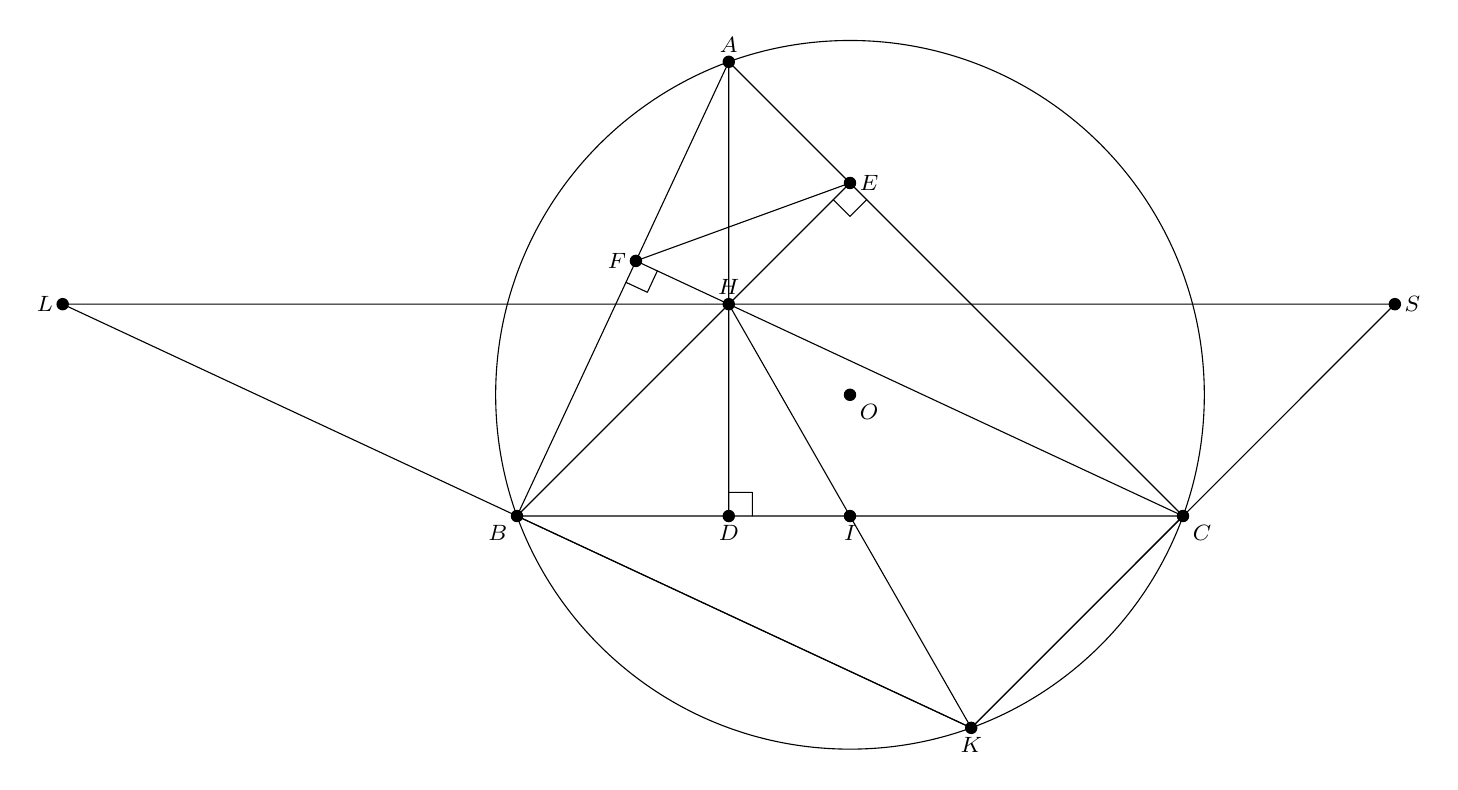
\begin{tikzpicture}[line join = round, line cap=round,>=stealth,font=\footnotesize,scale=1.5]
			\usetikzlibrary{calc,intersections,angles}
			
			% Khai báo hằng số
			\def\r{3} % r = 3cm
			
			% Định nghĩa tọa độ các điểm ban đầu
			\coordinate (O) at (0,0);
			\coordinate (B) at (-160:\r); 
			\coordinate (C) at (-20:\r);  
			\coordinate (A) at (110:\r); 
			
			% D là hình chiếu của A lên BC
			\coordinate (D) at ($(B)!(A)!(C)$);
			% E là hình chiếu của B lên AC
			\coordinate (E) at ($(A)!(B)!(C)$);
			% F là hình chiếu của C lên AB
			\coordinate (F) at ($(A)!(C)!(B)$);
			
			% H là giao điểm của BE và CF
			\path[name path=lineBE_H] (B) -- (E);
			\path[name path=lineCF_H] (C) -- (F);
			\path[name intersections={of=lineBE_H and lineCF_H, by=H}];
			
			% I là trung điểm của BC
			\coordinate (I) at ($(B)!0.5!(C)$);
			
			% Lấy điểm K sao cho O là trung điểm của AK (K = 2*O - A)
			\coordinate (K) at ($2*(O)-(A)$);
			% Lấy điểm L sao cho B là trung điểm của LK (L = 2*B - K)
			\coordinate (L) at ($2*(B)-(K)$);
			% Lấy điểm S sao cho C là trung điểm của SK (S = 2*C - K)
			\coordinate (S) at ($2*(C)-(K)$);
			
			% Vẽ các đối tượng hình học
			\draw (O) circle (\r);          % Đường tròn (O;r)
			\draw (A) -- (B) -- (K) -- (C) -- cycle; % Đa giác A-B-K-C-A (A-B-K-C là tứ giác, cycle sẽ nối C với A)
			\draw (B) -- (C) -- (F) -- (E) -- cycle; % Đa giác B-C-F-E-B
			\draw (A) -- (D);  
			\draw (L) -- (K);              % Đoạn A-D
			\draw (H) -- (K) -- (S) -- (L) -- cycle; % Đa giác H-K-S-L-K
			
			% Tô màu cho các điểm (theo cấu trúc đầu tiên)
			\fill (O) circle (1.5pt);
			\fill (A) circle (1.5pt);
			\fill (B) circle (1.5pt);
			\fill (C) circle (1.5pt);
			\fill (D) circle (1.5pt);
			\fill (E) circle (1.5pt);
			\fill (F) circle (1.5pt);
			\fill (H) circle (1.5pt);
			\fill (I) circle (1.5pt);
			\fill (K) circle (1.5pt);
			\fill (L) circle (1.5pt);
			\fill (S) circle (1.5pt);
			
			% Đặt nhãn cho các điểm (theo cấu trúc đầu tiên)
			\node[below right] at (O) {$O$};
			\node[above] at (A) {$A$};
			\node[below left] at (B) {$B$};
			\node[below right] at (C) {$C$};
			\node[below] at (D) {$D$};      
			\node[right] at (E) {$E$};      
			\node[left] at (F) {$F$};      
			\node[above] at (H) {$H$};      
			\node[below] at (I) {$I$};
			\node[below] at (K) {$K$};
			\node[left] at (L) {$L$};
			\node[right] at (S) {$S$};
			
			% Ký hiệu các góc vuông mới
			\pic[draw, angle radius=3mm]{right angle = B--F--C}; 
			\pic[draw, angle radius=3mm]{right angle = B--E--C}; 
			\pic[draw, angle radius=3mm]{right angle = A--D--C}; 
			
		\end{tikzpicture}
		
	\end{center}
	}
\end{ex}

\begin{ex} % Câu 14
	\begin{enumerate}
		\item[a)] Một cửa hàng có 80 sản phẩm. Người quản lý tính rằng nếu mỗi sản phẩm bán với giá 200 nghìn đồng thì tất cả sản phẩm đều bán hết. Biết rằng mỗi lần tăng giá thêm 20 nghìn đồng thì có thêm 4 sản phẩm không bán được. Hỏi người quản lý phải quyết định giá bán là bao nhiêu để thu nhập của cửa hàng là lớn nhất?
		\item[b)] Cho $a, b, c$ là các số dương thỏa mãn: $a \cdot b \cdot c = 1$.
		Tìm giá trị lớn nhất của biểu thức $P = \frac{1}{a+2b+3} + \frac{1}{b+2c+3} + \frac{1}{c+2a+3}$.
	\end{enumerate}
\end{ex}

\setcounterref{ex}{0}
